\documentclass[sigplan,screen]{acmart}

\AtBeginDocument{%
  \providecommand\BibTeX{{%
    \normalfont B\kern-0.5em{\scshape i\kern-0.25em b}\kern-0.8em\TeX}}}

\acmConference[CSE 158]{}{Assignment 2}{December 2023}
  
\begin{document}

\title{Decoding the Invisible: Bridging Latent Factors and Tags in Recommendation Systems}

\author{Zihan Liu}
\email{zil065@ucsd.edu}


\begin{abstract}
In this assignment, I mainly studies the ways to connect latent factors in 
recommendation systems to tags of items, allowing many cool additional features 
to be possible. There's very limited time around the final period when I stared 
this project so I couldn't go deeper to explore more models and applications, 
but I did my best to provide some interesting applications made possible by
some of the unique properties of these new models.
I know this paper is too long for this assignment, but
there's some very interesting application of this model in
the last section of result and conclusion. Make sure you check that out!
All code and latex source is available \href{https://github.com/anananan116/CSE158-Assignment2}{here}.
\end{abstract}


\maketitle

\section{Introduction}
\subsection{Introduction to the Topic}
The integration of latent factor models with item tags in recommendation systems marks a significant advancement in enhancing both interpretability and overall effectiveness. Traditional latent factor models, such as those described by Koren\cite{Koren09}, are adept at identifying patterns in user-item interactions but often suffer from a 'black-box' nature. This lack of transparency complicates the understanding of recommendation rationales for both users and system administrators, potentially undermining trust and engagement.

The absence of interpretability is a notable limitation, adversely affecting user trust and system transparency. It has been observed that users engage more actively with systems when they comprehend the mechanics of recommendations, especially how their contributions (like voting for tags) are utilized.\cite{Cosley07, Rashid02} Such understanding not only elevates user satisfaction but also facilitates more effective model tuning and troubleshooting. The inability to decipher the internal decision-making process of these models presents significant challenges in diagnosing and rectifying issues.\cite{KonstanRiedl12}

These models also grapple with challenges like the cold start problem, where accurately recommending new items or users with limited historical data is problematic. Tags provide an initial set of data points, enabling the system to make more informed initial recommendations.

This paper will explore solutions to these challenges by establishing connections between latent factors in traditional matrix factorization models and tags using predictive models such as linear regressors and random forests. These models will be employed to predict the presence of tags based on the latent factors of items. Furthermore, we will examine a novel model, tagMF\cite{LOEPP201921}, which generates latent factors for items based solely on the relevance of their tags, as opposed to the items themselves. The efficacy of this model in addressing the aforementioned problems will be demonstrated.

\subsection{Dataset Description}
In this study, we leverage a dataset initially gathered by Apurva Pathak, Kshitiz Gupta, and Julian McAuley, aimed at exploring bundle recommendations on the Steam platform\cite{Pathak17}. The datasets, available \href{https://cseweb.ucsd.edu/~jmcauley/datasets.html#steam_data}{here}, comprise two key components: one containing comprehensive game metadata \href{https://cseweb.ucsd.edu/~wckang/steam_games.json.gz}{(metadata)}, and another detailing user-game interaction data \href{https://datarepo.eng.ucsd.edu/mcauley_group/data/steam/australian_users_items.json.gz}{(interaction)}. The game metadata dataset includes detailed information on 10,978 games, encompassing aspects like user-voted tags, genres, pricing, release dates, and publishers. The interaction dataset, on the other hand, records around 5,000,000 instances of game purchases, coupled with the time users spent on each game. To optimize our study, we plan to filter out less popular games and inactive users. The methodology for this filtration, along with the corresponding data volumes pre- and post-cleaning, is summarized in \textbf{Table 1}.

\begin{table}
  \caption{Number of Data Points before and after Cleaning}
  \label{tab:freq}
  \begin{tabular}{ccl}
    \toprule
    Name of Data&Before Cleaning&After Cleaning\\
    \midrule
    Number of Users & 88,310 & 54,667\\
    Number of Games  & 32,134 & 1,656\\
    Number of Tags & 345 & 30/50/100\\
    Number of Interactions & 5,153,209 & 1,604,267\\
  \bottomrule
\end{tabular}
\end{table}

\begin{figure}[h]
  \centering
  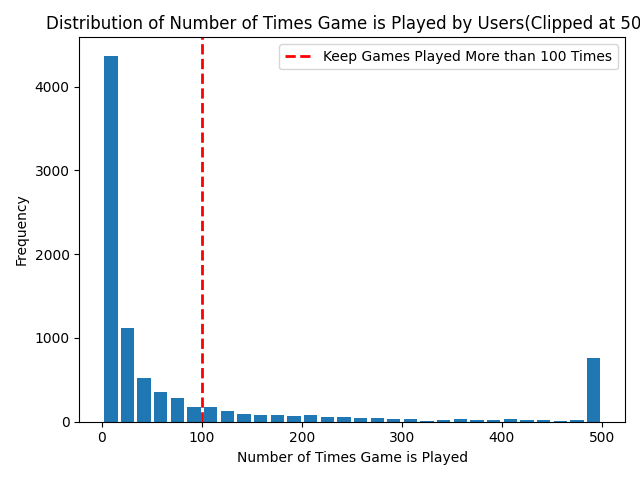
\includegraphics[width=\linewidth]{game_played_hist.png}
  \caption{Distribution of number of times games are played.}
\end{figure}
\subsection{Exploratory Data Analysis}

The data preprocessing phase of our study includes a strategic exclusion of less popular games. As depicted in \textbf{Figure 1}, we evaluate game popularity based on the number of instances a game is played for more than 60 minutes. Games that are played more than 100 times are selected for inclusion in our analysis. This criterion serves multiple purposes: it not only significantly reduces the volume of data for more efficient processing by the model but also helps in removing anomalies typically found in the data pertaining to less popular games. Furthermore, this approach enhances the focus on games with higher user engagement, which are more likely to yield insightful patterns for our study. Notably, integrating the excluded games back into the model for predictive analysis is found to be relatively straightforward, ensuring a comprehensive coverage in our model's applicability.

The selection of tags for our analysis is a crucial step in refining the dataset. To ensure relevance and representation, we conducted a frequency analysis of tag occurrences within the game metadata. The frequency distribution of tag appearances is meticulously documented in \textbf{Figure 2}. This data-driven approach enables us to identify and select the most frequently occurring tags for inclusion in our study. Furthermore, to comprehensively evaluate the performance of the tagMF model, we will experiment with varying numbers of tags. Also note here that the tags comes in order, the more people vote a tag, the index of it in the list of the metadata dataset is smaller. We will use this fact to assess the relevance of tags to games.

\begin{figure}[h]
  \centering
  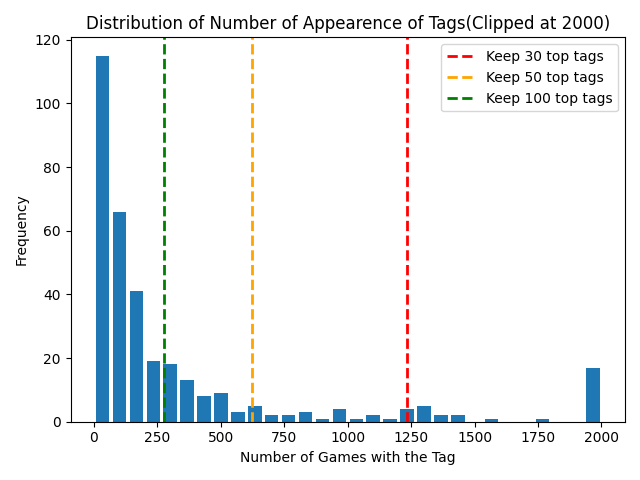
\includegraphics[width=\linewidth]{tag_appearnce_hist.png}
  \caption{Distribution of number of times tags appears in game metadata.}
\end{figure}

The next step in our exploratory analysis involves examining the pricing aspect of the games. Despite the absence of price-related information in the Steam tags, we can incorporate this crucial element manually by adding specific price-related tags to each game's tag list. To determine appropriate thresholds for price categorization, we analyzed the distribution of game prices, as detailed in \textbf{Figure 3}. Based on this analysis, we established three distinct price categories, represented by tags assigned at different price points. The thresholds for these tags are set at 0\$ (exclusive), 10\$, and 35\$. Each threshold signifies a different price range, allowing us to integrate price as a significant factor in our analysis. This inclusion of price tags is expected to enhance the richness of our dataset and provide more nuanced insights into user preferences and behavior in relation to game pricing.

\begin{figure}[h]
  \centering
  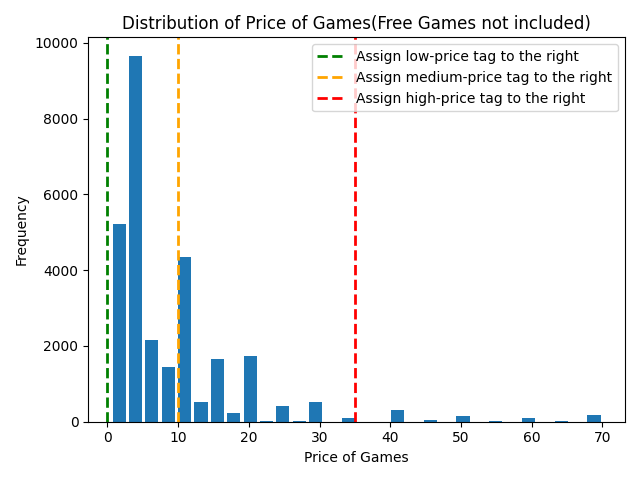
\includegraphics[width=\linewidth]{price_hist.png}
  \caption{Distribution of prices of games in game metadata.}
\end{figure}

\begin{table*}
  \caption{Example of $A_i$ for several games and tags}
  \label{tab:freq}
  \begin{tabular}{cccccl}
    \toprule
    Game & RPG & Simulation & Strategy & Anime & FPS\\
    \midrule
    Sid Meier’s Civilization® VI & 0.08 & 0.85 & 0.95 & 0.02 & 0.0\\
    Baldur's Gate 3 & 0.98 & 0.39 & 0.95 & 0.09 & 0.0\\
    NEKOPARA Vol. 1 & 0.11 & 0.45 & 0.01 & 1.0 & 1.0?\\
    Counter-Strike 2 & 0.01 & 0.32 & 0.36 & 0.06 & 1.0\\
  \bottomrule
\end{tabular}
\end{table*}

\section{Methodology and Data Preprocessing}
\subsection{Methodology}
The primary objective of this study is to explore the integration of tag information with latent factors in recommendation systems, aiming to address challenges like the cold start problem and the opaque nature of traditional latent factor models. While the focus is not primarily on prediction, the implementation of the biased tagMF model\cite{LOEPP201921}, akin to the traditional matrix factorization approach\cite{Koren09}, does result in real-value predictions. This approach aligns with the predictive task we undertook in assignment 1, which involved predicting the log-transformed playtime for specific user-game combinations.

Our methodology begins with fitting a biased latent factor model, incorporating both item and user factor matrices. We then use the item factor matrix as a feature set to predict tags for each game, which could only produce very limited results. Subsequently, we introduce the tagMF model. This model incorporates tags associated with each game into its structure, using the relevance of each tag to construct latent factors for games. The concept of tag relevance will be elaborated upon in the following section.

As both the tagMF and traditional latent factor models yield real-value predictions, we can initially compare their mean squared error (MSE) using various tag counts on a test dataset. Based on the findings in the original tagMF paper, we anticipate a slightly lower MSE for the tagMF model compared to the conventional latent factor approach. This comparison should validate the predictive accuracy of the tagMF model.

Beyond predictive performance, we aim to demonstrate how the tagMF model addresses the cold start problem and enhances interpretability of latent factors through the analysis of tag weights. This aspect will further corroborate the model's effectiveness in mitigating issues associated with the 'black-box' nature of traditional latent factor models.

\subsection{Data Preprocessing}
The initial preprocessing step, as outlined in the EDA section, involves pruning our dataset by removing unpopular games, inactive users, and excess tags. This might appear to be a significant reduction, yet it's crucial to recognize that many games in the dataset were played by a sparse user base, and there were users who hadn't purchased any games. Focusing on more active components of the dataset allows the model to learn from data that is most representative of general user behavior. Additionally, integrating these excluded elements into the tagMF model later is a relatively straightforward process.

The tagMF model\cite{LOEPP201921} necessitates an additional input – a relevance matrix between tags and games, denoted as $A_i \in \mathbb{R}^{|T| \times |I|}$, where $T$ symbolizes the set of tags utilized in the model, and $I$ represents the collection of games. Each matrix column correlates a single game with the relevance of each tag used in the model. An exemplar of this matrix is demonstrated in \textbf{Table 2}. The relevance score, lying in the continuous range of [0,1], reflects how pertinent a tag is to a game, with higher scores indicating greater relevance.

For our dataset, the tag order in the game metadata informs the relevance scores. Tags appearing earlier, hence voted by a larger number of users, are considered more relevant. These scores are calculated using the relative position of the tag ($\text{game\_tags.index(tag)} / \text{len(game\_tags)}$), modified by an inverse Gamma transformation with $\gamma=3$, as illustrated in \textbf{Figure 4}. A rarity bonus is added to less common tags, acknowledging their potential significance to a game. The overall relevance score is a sum of these components, defaulting to zero for tags not present in a game’s metadata.

\begin{figure}[h]
  \centering
  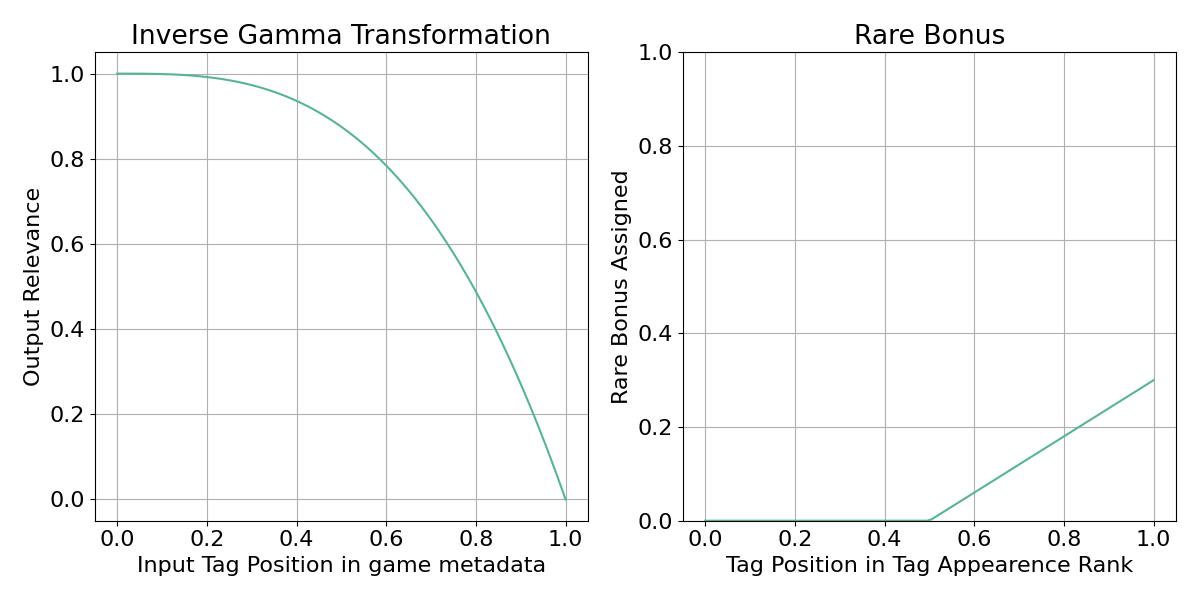
\includegraphics[width=\linewidth]{transformation.png}
  \caption{Transformation Applied to gain tag reference(Left) and Rare Tag Bonus assignment rule(Right)}
\end{figure}

Furthermore, the relevance matrix can incorporate features beyond the game's original tags. For instance, I included game prices by adding three non-original Steam tags, as detailed in the EDA. Assigning relevance scores to these manually added tags, based on their distance from predetermined thresholds, could further enhance the model's effectiveness. Thus, any continuous feature can be integrated by setting appropriate thresholds for new tags and associating the distance between the feature and these thresholds with each tag’s relevance. Additionally, discrete or binary features can be directly encoded as tags, though an excessive number might affect the model’s efficiency.

\section{Model Structure and evaluations}
This section outlines the construction, evaluation, and practical application of our models. We commence by constructing a biased latent factor model as delineated by Koren\cite{Koren09}. The model is defined by the following equation:
\begin{equation}
  r_{u,i} \approx \alpha + \beta_u + \beta_i + \gamma_u \cdot \gamma_i
\end{equation}
where \(\alpha\) represents the global offset, \(\beta_u\) and \(\beta_i\) denote the user and item offsets, respectively, and \(\gamma_u\), \(\gamma_i\) are the latent factors for the user and item.

\subsection{Predicting Tags Using Latent Factors as Features}
Rather than transitioning directly to an entirely new model, a logical step is to develop a supplementary model that links the item's latent factors to its tags. Specifically, for each tag, we can train a model using \(\gamma_i\) of an item as input, predicting a binary outcome indicating the tag's presence. An initial approach using a logistic regressor yielded approximately 87\% accuracy on the test set. While impressive, this result is somewhat misleading as the tags' distribution is heavily skewed, allowing for roughly 85\% accuracy by consistently predicting False.

Subsequent experiments with other models, including random forests and neural networks, did not significantly outperform the logistic regressor. Given that this exploration primarily aims to demonstrate the impracticality of directly correlating latent factors from matrix factorization models with tags, a detailed exposition of these model implementations is omitted. The failure of these methods could be attributed to the latent factors encapsulating implicit item information not present in the tags, or the basic nature of these models being unsuitable for this specific challenge. Thus, directly linking latent factors with tags is not an issue readily resolved through trial-and-error with connecting models. However, by reconceptualizing tags as the bridge between items and latent factors, we can seamlessly integrate this idea into the model framework, offering a more cohesive approach.

\subsection{tagMF Model}

In this study, we have implemented and tested the tagMF model in its biased form, originally proposed by Loepp et al. \cite{LOEPP201921} and based on the approach by Forbes and Zhu \cite{ForbesZhu11}. The model's structure is described using a notation system that aligns with what we learned in class, though it may differ slightly from the one used in the original paper. A key aspect of our approach is the construction of a relevance matrix \(A_i\), connecting each game with its relevance to each tag. Concurrently, we posit the existence of a matrix \(A_u \in \mathbb{R}^{|T| \times |U|}\), where \(T\) represents the set of tags and \(U\) the set of users. The traditional matrix factorization model, typically represented as \(R \approx U V^T\), is redefined in our approach as:

\begin{equation}
  R \approx U V^T = A_u \Theta_u (A_i \Theta_i)^T
\end{equation}

In this formulation, the item factors \(V\) are constructed entirely through their relevance with tags, achieved by multiplying the relevance matrix \(A_i\) with \(\Theta_i \in \mathbb{R}^{|T| \times |F|}\). The user factors, represented by \(\Theta_u \in \mathbb{R}^{|T| \times |F|}\), are similarly defined. This method effectively transforms the tag relevance vectors into latent factors, akin to those used in conventional SVD models.

One challenge we face is constructing the matrix \(A_u\). While one might consider building \(A_u\) using existing interaction data between users and games, in our training approach, we treat \(A_u\Theta_u\) as a single entity, similar to \(U\) in traditional SVD models. Despite this amalgamation during training, the underlying assumption that \(U = A_u\Theta_u\) still holds. We revisit the separate components, \(A_u\) and \(\Theta_u\), after the model is trained.

To account for the relative nature of game playtime to both players and games, we reintegrate global and user/item offsets into our model. The term \(U(A_i \Theta_i)^T\) is utilized as an estimate of a user's interest in games, forming the basis for recommendations. The final prediction model is given by:

\begin{equation}
  r_{u,i} \approx \alpha + \beta_u + \beta_i + \gamma_u^T\Theta_i^Ta_i
\end{equation}

In this equation, \(\gamma_u\) denotes a row from \(U\), and \(a_i\) a row from \(A_i\) corresponding to a specific user-item pair \((u,i)\). The minimization problem, following Forbes and Zhu\cite{ForbesZhu11}, is expressed as:

\begin{equation}
 \text{arg min}_{U, \Theta_i} \sum_{(u,i)} (r_{ui} - (\alpha + \beta_u + \beta_i + \gamma_u^T\Theta_i^Ta_i))^2 + \text{reg}
\end{equation}

The regularization term, \(\text{reg}\), is formulated as:

\begin{equation}
 \text{reg} = \lambda \left(\sum_u \beta_u^2 + \sum_i \beta_i^2 + \sum_u \lVert \gamma_u \rVert^2 + \lVert \Theta_i \rVert^2\right)
\end{equation}

A detailed discussion on the gradient descent algorithm is omitted, as TensorFlow handles this aspect. My complete implementation, including data preprocessing and applications of the model, is accessible \href{https://github.com/anananan116/CSE158-Assignment2}{here}.
\subsection{Evaluation}
In evaluating the performance of the tagMF and conventional matrix factorization (MF) models, I conducted a detailed analysis considering various parameters such as the number of tags, lambda values, and the number of iterations. This evaluation was based on the mean squared error (MSE) as a performance metric, averaged over 10 models trained under the same settings.

\begin{figure}[h]
  \centering
  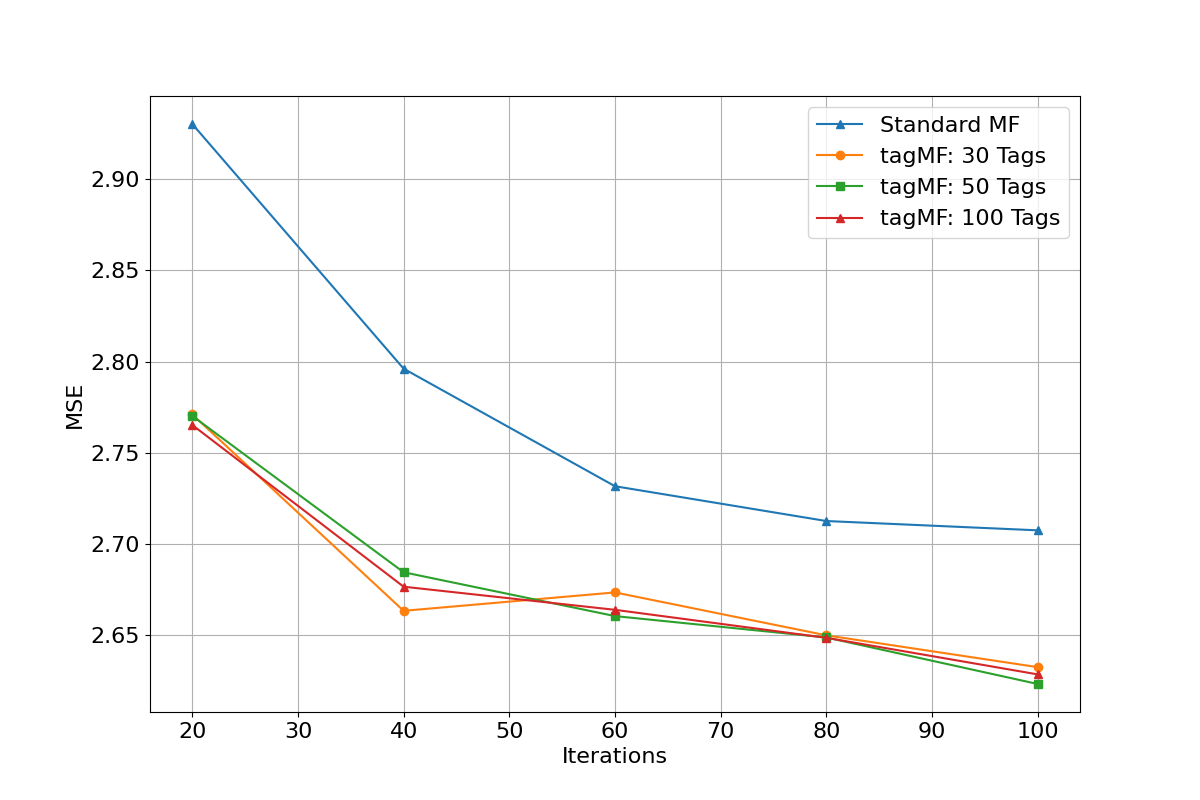
\includegraphics[width=\linewidth]{evaluation_1.png}
  \caption{Performance comparison of conventional MF and tagMF models.}
\end{figure}

Our initial comparison between the conventional latent factor model and the tagMF models, as depicted in \textbf{Figure 5}, reveals that the tagMF model outperforms the standard MF model by about 3\%. This improvement is primarily attributed to the additional information (tags) utilized in the tagMF model. This performance enhancement aligns closely with the results observed by Loepp et al. \cite{LOEPP201921}, who reported a similar boost of around 3.7\%. Notably, the tagMF model's performance improved with an increasing number of tags (30, 50, 100). Specifically, the models with 50 and 100 tags consistently outperformed the 30-tag model, although the 50-tag model showed a slight edge over the 100-tag version. This could be due to the lesser relevance of additional tags in the dataset, as they appeared infrequently in the training data (refer to the EDA section for detailed tag appearance counts, which use all game in original dataset to count tag appearance, the number of appearance should be even less after data cleaning on training data.). Enhanced feature engineering and more domain-specific knowledge in assigning tag relevance could further improve the model's performance, especially when incorporating rare tags.

\begin{figure}[h]
  \centering
  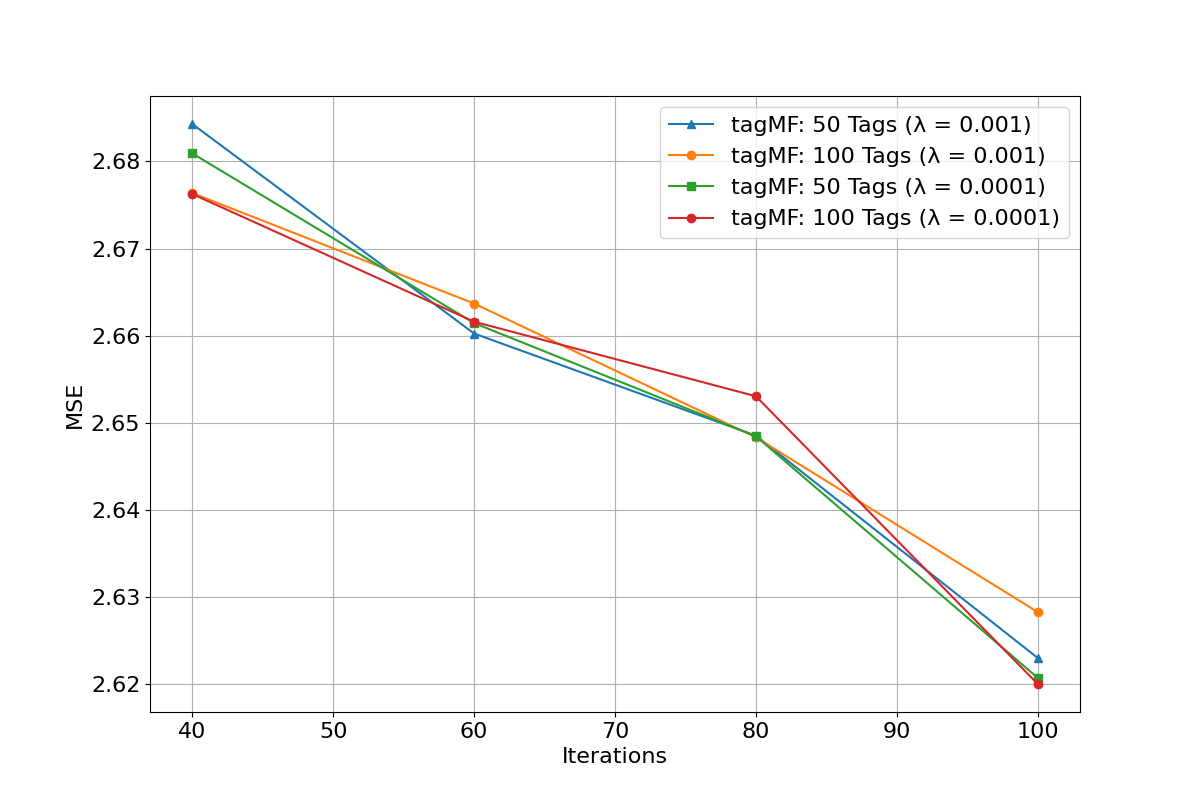
\includegraphics[width=\linewidth]{evaluation_2.png}
  \caption{Impact of lambda values on tagMF model performance.}
\end{figure}

Furthermore, as illustrated in \textbf{Figure 6}, we assessed the impact of different lambda values on the tagMF model. The analysis indicates that the model's performance was not significantly affected by varying lambda values. This observation supports Loepp et al.'s \cite{LOEPP201921} assertion that the tagMF system is more resistant to overfitting compared to conventional latent factor models.

In summary, the tagMF model not only showed superior performance compared to the conventional MF model but also demonstrated the benefit of incorporating additional information through tags. The model's robustness against overfitting and its sensitivity to the number of tags used further highlight its potential in complex user-game interaction scenarios.

\section{Related work}

The research presented in this paper is inspired by and builds upon a series of influential works in the field of recommendation systems. The integration of latent factor models with item tags, a core aspect of this study, draws heavily from the foundational concepts established in the seminal work of Koren\cite{Koren09}. Koren's exploration into latent factor models, particularly in the context of user-item interactions, laid the groundwork for understanding the potential and limitations of these models in recommendation systems.

The challenge of interpretability in recommendation systems, as highlighted by Cosley et al.\cite{Cosley07} and Rashid et al.\cite{Rashid02}, has been a critical influence in shaping the direction of this research. Their observations regarding the importance of user engagement and understanding in the context of recommendation systems underscore the need for models that are not only effective but also transparent and explainable to users.

The tagMF model, central to this study, is directly inspired by the innovative work of Loepp et al.\cite{LOEPP201921}. Their approach to integrating tag information into latent factor models to enhance interpretability and address problems like the cold start issue has been a pivotal reference for this research. The adoption and adaptation of their model to the specific context of Steam game recommendations, as originally compiled in the dataset by Pathak, Gupta, and McAuley\cite{Pathak17}, demonstrate the practical application of these theoretical concepts in a real-world scenario.

This research also delves into the realm of predictive modeling, employing techniques such as linear regressors and random forests to establish connections between latent factors and item tags. The exploration of these models, although not as successful as the tagMF model in this context, provided valuable insights into the complexities and challenges inherent in bridging latent factors with explicit item characteristics like tags. I also found some other researches from Rossetti et al.\cite{Rossetti13} and Kunkel et al.\cite{kunkel18} that offers significant insights into enhancing the interpretability and effectiveness of latent factor models in recommendation systems using connection between latent factors and other features of items.

The study by Rossetti et al. \cite{Rossetti13} delves into advanced methods for improving the interpretability of latent factors in collaborative filtering models. It emphasizes the potential of leveraging textual data associated with items, such as product descriptions or user reviews, to elucidate the latent factors derived from user-item interactions. This approach is congruent with the aim of this research, which involves marrying latent factors with item tags to bolster the transparency and comprehensibility of the recommendation process.

In Kunkel et al.'s work\cite{kunkel18}, the authors explore integrating topic modeling techniques, particularly Latent Dirichlet Allocation (LDA), with latent factor models to analyze textual data related to items. This method seeks to establish correlations between textual topics and latent factors, offering a nuanced understanding of the relationship between item attributes and user preferences. This exploration is particularly pertinent to the current research, as it exemplifies a methodology to connect the latent factors of items with their distinct characteristics, akin to the use of tags in this study.

In conclusion, this paper represents a comprehensive synthesis of methodologies and ideas from pivotal contributions in the field of recommendation systems. It aims to address existing challenges and advance the understanding of model interpretability and user engagement, thereby pushing the boundaries of what is achievable in recommendation systems.


\begin{table*}
  \caption{Top 10 Games Recommended for Selected Tags: Simulation, Strategy, Sci-Fi}
  \label{tab:freq}
  \begin{tabular}{cll}
    \toprule
    Rank of Recommendation & Link to Recommended item & Recommendation Score\\
    \midrule
    1 & \url{https://store.steampowered.com/app/294100} & 11.195\\
    2 & \url{https://store.steampowered.com/app/342200} & 10.851\\
    3 & \url{https://store.steampowered.com/app/223830} & 10.410\\
    4 & \url{https://store.steampowered.com/app/208140} & 10.259\\
    5 & \url{https://store.steampowered.com/app/8500}   & 10.236\\
    6 & \url{https://store.steampowered.com/app/65980}  & 10.105\\
    7 & \url{https://store.steampowered.com/app/212680} & 10.065\\
    8 & \url{https://store.steampowered.com/app/322910} & 9.968\\
    9 & \url{https://store.steampowered.com/app/301520} & 9.943\\
    10 & \url{https://store.steampowered.com/app/290300} & 9.893\\
  \bottomrule
\end{tabular}
\end{table*}

\section{Result and Conclusion}

\subsection{Application}
As we discussed in the very beginning, the conventional SVD models suffer from the lack of interpretability and cold start problem, we will first see how tagFM could solve those problems 
\subsubsection{Model interpretability}

The tagMF model's capability to extract and analyze the tags-to-latent-factor matrix, \(\Theta_i\), presents a significant advantage in understanding the model's decision-making process. While a heatmap visualization of this matrix (\textbf{Figure 7}) aids readers in grasping its structure, the real value lies in analyzing the matrix itself. The weights assigned to each tag within \(\Theta_i\) reveal how tags influence the formation of latent factors, offering deep insights into the model’s inner workings.

\begin{figure}[h]
  \centering
  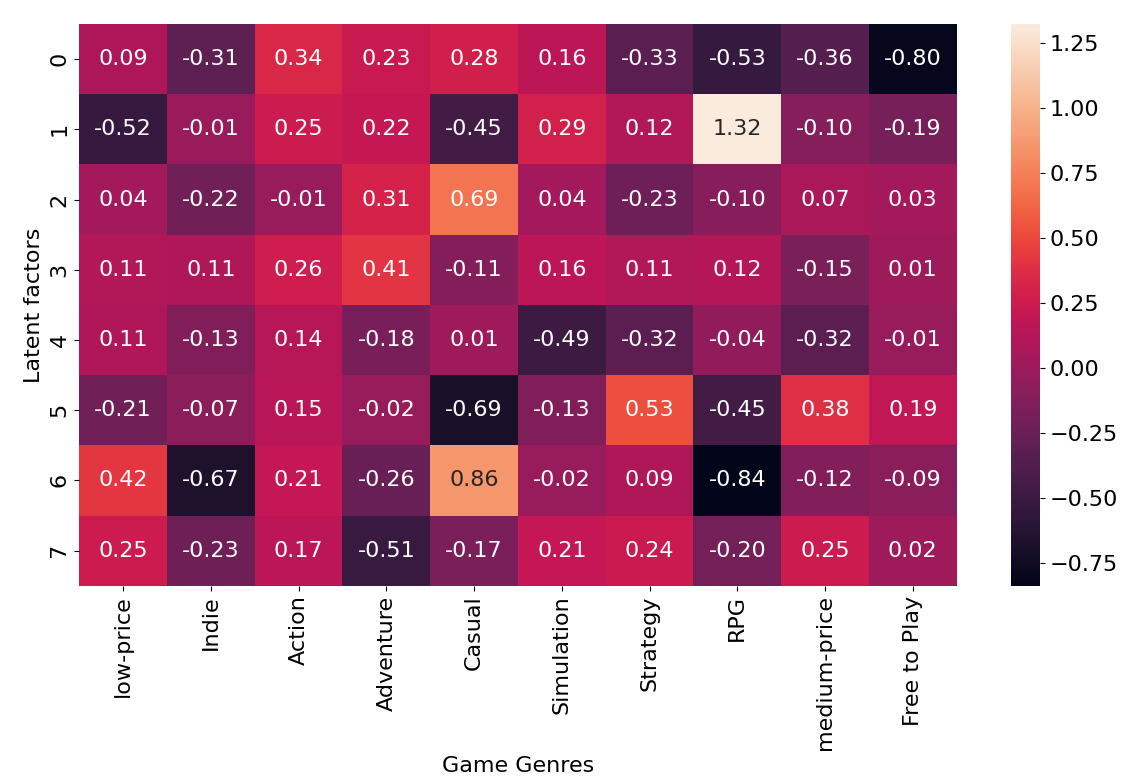
\includegraphics[width=\linewidth]{relationship.png}
  \caption{Heatmap for relationship between tag relevance and latent factors ($\Theta_i$), only displaying top 10 tags and first 8 latent factors}
\end{figure}

This analysis is pivotal for enhancing model interpretability and enabling effective tuning. By identifying how specific tags contribute to recommendations, adjustments can be made to optimize the model’s performance and address potential biases. Furthermore, understanding these relationships between tags and latent factors provides valuable insights into user preferences, guiding content strategy and enhancing the transparency of recommendations. This feature of the tagMF model thus plays a crucial role in advancing the interpretability and efficacy of recommendation systems.

\subsubsection{Cold Start Problem}
As previously discussed, conventional Singular Value Decomposition (SVD) methods in recommendation systems often struggle with the cold start problem, particularly when a new user joins and lacks interaction data. Many commercial systems resort to simpler recommendation strategies in such cases, typically suggesting the most popular items\cite{KonstanRiedl12} or relying on similarity functions of user-selected tags item tags for recommendations, which do not fully leverage pre-trained models.

The tagMF model offers a novel solution to this problem by utilizing its existing structure to recommend items to new users based solely on their tag preferences. To achieve that, we eventually need to estimate the user's latent factors $\gamma_u$, but keep in mind that the assumption that $U = A_u\Theta_u$  still stands even though we did not train the parameters of $A_u\Theta_u$. Firstly, a user's relevance to tags, \(a_u\), is generated by assigning a value of 1 to selected tags and 0 to others. Then, since both item and user preferences are mapped to the same latent factor space, each factor is assumed to reflect a latent characteristic with the same semantic meaning for users and items\cite{Koren09, LOEPP201921, Donkers16}. We then use the assumption that \(\Theta_u\) is equivalent to \(\Theta_i\) to estimate \(\gamma_u\) using \(\Theta_i\):

\begin{equation}
 \gamma_u = a_u \Theta_i
\end{equation}

The recommendation score for each item \(i\) is calculated as:

\begin{equation}
\text{score} = \gamma_u^T\Theta_i^Ta_i = a_u\Theta_i(a_i\Theta_i)^T
\end{equation}

By ranking these scores, we can generate recommendations for new users without interaction data. An example set of recommendations generated by the tagMF model with 30 tags and selected tags of Simulation, Strategy, and Sci-Fi is presented in \textbf{Table 3}. You can click on the links to see their Steam page and check yourself if you are a game enthusiast, but I've checked for you and all of them are perfect matches for the input tags. (The dataset only contains games that publishes before 2019, thus more old games are recommended.)

Furthermore, the \(\gamma_u\) generated for a new user can be normalized and added to the model parameters (\(U\)) after it is normalized to similar scale as other user factors, allowing the system to refine recommendations as more interaction data becomes available. This method opens up possibilities for more applications, such as a tag-based recommendation system where users can select preferred tags and specify tag relevance scores. Then we pretend this input as a user's relevance score and do exactly the same as above to get recommendations for given tags and relevance.

\subsection{Refinements and Future Outlook}

\subsubsection{Enhancing Tag Relevance Assignment}
One critical area for refinement in the model is the assignment of tag relevance for items. Currently, the relevance is determined without specific data on the number of user votes per tag. Incorporating this data could significantly enhance the accuracy of tag relevance assignment. For instance, tags with a higher number of votes could be given more weight, reflecting their broader acceptance or popularity among users.

Additionally, the model sometimes produces skewed recommendations when rare tags are included. This could be attributed to these tags often being associated with outlier items in the dataset. Therefore, a more nuanced approach is needed to handle rare tags. Careful analysis and consideration should be given to how these tags are weighted and interpreted by the model to improve recommendation accuracy, especially in cases where rare tags are involved.

\subsubsection{Considering Bayesian Personalized Ranking (BPR) for Recommendations}
Another potential direction for future development is the exploration of Bayesian Personalized Ranking (BPR) in the recommendation system. Unlike the current latent factor model structure, BPR focuses more directly on user-item interactions, specifically on the purchase history. This approach could lead to more accurate and reasonable recommendations, as it is grounded in actual user behavior rather than just inferred preferences.

While BPR may provide more targeted recommendations, it's important to note that some information might be lost in this transition. Specifically, data regarding the duration a game is played, which can be an indicator of user preference intensity, might not be fully utilized in a BPR framework. Nevertheless, BPR's emphasis on direct interactions makes it a promising alternative for future iterations of the recommendation system. We can simply replace the $\gamma_i$ in BPR model to $\Theta_ia_i$ to form the tagMF version of BPR.

In summary, the ongoing development of this recommendation model should focus on refining the assignment of tag relevance and possibly adopting a BPR-based approach. These changes aim to enhance the accuracy and relevance of recommendations, catering more closely to user preferences and behaviors.

\subsection{Conclusion}

This paper has embarked on an explorative journey to integrate latent factors in recommendation systems with item tags, a venture that transcends the confines of a typical predictive task. Despite the time constraints around the project's final phase, we have managed to implement and showcase a model that not only adheres to but also outperforms some of the baseline models discussed in class. The tagMF model, inspired by pioneering works in the field\cite{LOEPP201921}, has demonstrated its efficacy in enhancing interpretability and addressing the cold start problem, typical of conventional SVD methods.

Our exploration into the realms of model interpretability and handling the cold start problem has unveiled novel applications of the tagMF model. The ability to visualize and analyze the tags-to-latent-factor matrix (\(\Theta_i\)) not only enhances our understanding of the model's decision-making process but also opens new avenues for model tuning and user insight. This has been particularly beneficial in addressing the lack of interpretability and troubleshooting challenges in traditional latent factor models.

Furthermore, the model's unique structure has allowed for innovative solutions to the cold start problem. By leveraging tag preferences of new users and the assumption that \(U = A_u\Theta_u\), the model can generate personalized recommendations even without prior user-item interaction data. This approach not only addresses a critical limitation in traditional models but also enhances the user experience from the outset.

Looking forward, the refinement of tag relevance assignment and the potential adoption of Bayesian Personalized Ranking (BPR) suggest exciting possibilities for future development. These enhancements, aimed at improving the accuracy and relevance of recommendations, highlight the evolving nature of recommendation systems and their increasing alignment with user preferences and behaviors.

In conclusion, this assignment has not only been a fulfillment of academic requirements but also a meaningful exploration into the potential of modern recommendation systems. It highlights the importance of continuous innovation and adaptation in the field, driven by the ever-changing landscape of user needs and technological advancements. Happy reviewing!



%%
%% The next two lines define the bibliography style to be used, and
%% the bibliography file.
\bibliographystyle{ACM-Reference-Format}
\bibliography{assignment2_bib}

%%
%% If your work has an appendix, this is the place to put it.
\appendix

\end{document}
\endinput
%%
%% End of file `sample-sigplan.tex'.
